\documentclass{article}

\usepackage{minitoc}
\usepackage{tabularx}
\usepackage{booktabs}
\usepackage{graphicx}
\usepackage{hyperref}
\usepackage{xcolor}
\usepackage{blkarray}
\usepackage{amsthm, amssymb, amsmath}
\usepackage{caption}
\usepackage{subcaption}
\usepackage{multirow}
\usepackage{multicol}
\usepackage[ruled,vlined]{algorithm2e}

\usepackage{natbib}
\bibliographystyle{abbrvnat}

\theoremstyle{definition}
\newtheorem{definition}{Definition}[section]
\newtheorem{theorem}{Theorem}[section]
\newtheorem{lemma}[theorem]{Lemma}
\newtheorem{conjecture}[theorem]{Conjecture}
\newtheorem{Prop}{Proposition}

\usepackage[margin=2.5cm, includefoot, footskip=30pt]{geometry}
\pagestyle{plain}
\setlength{\parindent}{0em}
\setlength{\parskip}{1em}

\renewcommand{\baselinestretch}{1}

\usepackage{standalone}

\newtheorem{proposition}{Proposition}

\title{Reactive strategies with longer memory}

\author{Nikoleta E. Glynatsi, Ethan Akin, Martin Nowak, Christian Hilbe}
\date{}

\begin{document}

\maketitle

\section{Formal Model}

We consider infinitely repeated games among two players, player $p$ and
player $q$. Each round, they engage in the donation game with payoff matrix

\begin{equation} \label{Eq:DonationGame}
\left(
\begin{array}{cc}
b-c	&-c\\
b	&0
\end{array}
\right).
\end{equation}

Here $b$ and $c$ denote the benefit and the cost of cooperation, respectively. 
We assume $b\!>\!c\!>\!0$ throughout.
Therefore, payoff matrix~\eqref{Eq:DonationGame} is a special case of the
prisoner's dilemma with payoff matrix,

\begin{equation} \label{Eq:PrisonerDilemma}
    \left(
    \begin{array}{cc}
    R & S\\
    T & P
    \end{array}
    \right),
\end{equation}

where $T > R > S > P$ and $2 R > T + S$. Here, $R$ is the reward payoff of mutual
cooperation, $T$ is the temptation to defect payoff, $S$ is the sucker's payoff,
and $P$ is the punishment payoff for mutual defection.

We assume in the following, that the players' decisions only depend on the
outcome of the previous $n$ rounds. To this end, an {\it $n$-history for player
$p$} is a string $h^p=(a^p_{-1},\ldots,a^p_{-n})\!\in\!\{C,D\}^n$. An entry
$a^p_{-k}$ corresponds to player $p$'s action $k$ rounds ago. Let $H^p$ denote
the space of all $n$-histories of player~$p$. Analogously, let $H^q$ as the set
of $n$-histories $h^q$ of player~$q$. Sets $H^p$ and $H^q$ contain
$|H^p|=|H^q|=2^{n}$ elements each.

A pair $h\!=\!(h^p,h^q)$ is called an {\it $n$-history of the game}. We use
$H=H^p\times H^q$ to denote the space of all such histories. This set contains
$|H|=2^{2n}$ elements.

{\bf Memory-$n$ strategies.} A {\it memory-$n$} strategy is a vector
$\mathbf{m}=(m_h)_{h\in H}\in[0,1]^{2n}$. Each entry $m_h$ corresponds to the
player's cooperation probability in the next round, depending on the outcome of
the previous $n$ rounds. If the two players use memory-$n$ strategies
$\mathbf{m}$ and $\mathbf{m'}$, one can represent the interaction as a Markov
chain with a $2^{2n}\!\times\!2^{2n}$ transition matrix $M$. Let
$\mathbf{v}=(v_h)_{h\in H}$ be an invariant distribution of this Markov chain.
Based on the invariant distribution $\mathbf{v}$, we can also compute the
players' payoffs. To this end, let $\mathbf{S}^k = (S_h^k)_{h\in H}$ denote the
vector that returns for each $h$ the one-shot payoff that player $p$ obtained
$k$ rounds ago,

\begin{equation}
    S_h^k = \left\{
    \begin{array}{cl}
    b-c	&\text{if}~ a_{-k}^p=C~\text{and}~ a_{-k}^q=C\\
    -c	&\text{if}~ a_{-k}^p=C~\text{and}~ a_{-k}^q=D\\
    b	&\text{if}~ a_{-k}^p=D~\text{and}~ a_{-k}^q=C\\
    0	&\text{if}~ a_{-k}^p=D~\text{and}~ a_{-k}^q=D
    \end{array}
    \right.
\end{equation}

Then we can define player $p$'s repeated-game payoff $s_{\mathbf{m},\mathbf{m'}}$ as

\begin{equation} \label{Eq:Payoff}
s_{\mathbf{m},\mathbf{m'}}  = \mathbf{v}\cdot \mathbf{S}^1 = \mathbf{v}\cdot \mathbf{S}^2 = \ldots = \mathbf{v} \cdot \mathbf{S}^n.
\end{equation}

The equalities $\mathbf{v}\cdot \mathbf{S}^1 = \ldots = \mathbf{v} \cdot
\mathbf{S}^n$ correspond to the intuition that it does not matter which of the
past $n$ rounds we use to define average payoffs. The payoff
$s_{\mathbf{m'},\mathbf{m}}$ of player $q$ can be defined analogously.

Let's provide definitions for some additional terms that will be used in this
manuscript.

{\bf Nash Strategies.} A strategy $\mathbf{m}$ for player $p$, is a \textit{Nash
strategy}, if player $q$ never receives a payoff higher than that of the mutual
cooperation payoff. Irrespective of $q$'s strategy. Namely if,

\begin{equation}\label{Eq:Nash}
    s_{\mathbf{m'},\mathbf{m}} \leq (b - c) \; \forall \; m' \; \in [0, 1]^{2n}.
\end{equation}

{\bf Nice Strategies.} A player's strategy is \textit{nice}, if the player is
never the first to defect. A nice strategy against itself receives the
mutual cooperation payoff, $(b - c)$.

{\bf Partner Strategies.} For player $p$, a \textit{partner strategy} is a strategy
which is both nice and Nash.

Partners strategies are of interest because they are strategies that strive to
achieve the mutual cooperation payoff of $(b - c)$ with their co-player.
However, if the co-player doesn't cooperate, they are prepared to penalize them
with lower payoffs. Partner strategies, by definition, are best responses to
themselves, making them Nash strategies~\citep{Hilbe:GEB:2015}. All partner
strategies are Nash strategies, but not all Nash strategies are partner
strategies.

Previously, the work of~\citep{akin:EGADS:2016} characterized all partner strategies in the
case of memory-one strategies. For higher memory values ($n > 1$), a few works
(\citep{hilbe:PNAS:2017}) have managed to characterize subsets of memory$-n$ partner
strategies. This difficulty arises from the fact that as memory increases,
obtaining analytical results becomes more challenging. In this work, we focus on
reactive strategies instead of memory$-n$ strategies. Reactive strategies, a
subset of memory$-n$ strategies, are formally introduced in Section~\ref{section:reactive_strategies}. We
characterize all reactive partner strategies for $n = 2$ and $n = 3$, and present a
series of results starting from Section~\ref{section:self_reactive_sufficiency}. In the following section, we will
discuss a series of results for the case of memory$-n$.

\section{An Extension of Akin's Lemma}

\textbf{Akin's Lemma.} The work of~\citep{akin:EGADS:2016} focuses on the case of
memory-one strategies, thus for $n=1$. A memory-one strategy of player $p$ is
represented by the vector $\mathbf{m} = (m_1, m_2, m_3, m_4)$, and and when
played against a co-player with strategy $\mathbf{m}'$, the resulting stationary
distribution is denoted as $\mathbf{v} = (v_1, v_2, v_3, v_4)$. Akin's lemma
states the following,

\begin{lemma}[Akin's Lemma]\label{lemma:akin}

Assume that player \(p\) uses the memory-one strategy \(\mathbf{m}=(m_1, m_2,
m_3, m_4)\), and \(q\) uses a strategy that leads to a sequence of distributions
\(\{\mathbf{v}^{k}, k = 1, 2, ...\}\) with \(\mathbf{v}^{k}\) representing the
distribution over the states in the \(k^{\text{th}}\) round of the game. Let
\(\mathbf{v}\) be the associated stationary distribution, then,

    \begin{align}
      \lim_{n \rightarrow \infty} \frac{1}{n} \sum_{k=1}^{n} \mathbf{v}^{k} \cdot (\mathbf{m} - (1, 1, 0 , 0)) & = 0, \text{ and therefore } \mathbf{v} \cdot (\mathbf{m} - (1, 1, 0, 0)) = 0.
    \end{align}
\end{lemma}

\textbf{Akin's Lemma for $1\!\le\!k\!\le\!n$.}

One special case of memory$-n$ strategies are the round$-k-$repeat strategies for
some $1\!\le\!k\!\le\!n$. Player $p$ uses a
{\it round-$k$-repeat strategy} $\mathbf{m}^{k-\text{Rep}}$ if in any given
round, the player chooses the same action as $k$ rounds ago. That is, if the
game's $n$-history is such that $a^p_{-k}\!=\!C$, then
$m^{k-\text{Rep}}_h\!=\!1$; otherwise $m^{k-\text{Rep}}_h\!=\!0$.

With the same method as in \citep{akin:EGADS:2016}, one can show {\it Akin's
Lemma}: For each $k$ with $1\!\le\!k\!\le\!n$, the invariant distribution
$\mathbf{v}$ satisfies the following relationship,

\begin{equation} \label{Eq:AkinsLemma}
\mathbf{v} \cdot (\mathbf{m}-\mathbf{m}^{k-\text{Rep}}) \!=\! \sum_{h\in H} v_h (m_h-m_h^{k-\text{Rep}}) = 0.
\end{equation}

The intuition for this result is that $\mathbf{v}\cdot \mathbf{m}$ and all
$\mathbf{v}\cdot \mathbf{m}^{k-\text{Rep}}$ are just different (but equivalent)
expressions for player $p$'s average cooperation rate. For example,
$\mathbf{v}\cdot\mathbf{m}$ corresponds to a setup in which one first draws a
history $h$ according to the invariant distribution $\mathbf{v}$; then one takes
player $p$'s probability $m_h$ to cooperate in the next round; the expectation
of this procedure is $\sum_{h\in H} v_h m_h$.

{\bf \%ToDo} Do we need a proof here? The intuition is summarising the proof.

\noindent
{\bf Zero-determinant strategies.}
Based on Akin's Lemma, we can derive a theory of zero-determinant strategies
analogous to the case of memory-one strategies. In the following, we say a
memory-$n$ strategy $\mathbf{m}$ is a zero-determinant strategy if there are
$k_1$, $k_2$, $k_3$ and $\alpha$, $\beta$, $\gamma$ such that $\mathbf{m}$ can
be written as

\begin{equation} \label{Eq:DefZD}
\mathbf{m} = \alpha \mathbf{S}^{k_1} + \beta \mathbf{\tilde{S}}^{k_2} + \gamma \mathbf{1} + \mathbf{m}^{k-\text{Rep}},  
\end{equation} 
where $\mathbf{1}$ is the vector for which every entry is 1. By Akin's Lemma and the definition of payoffs,
\begin{equation} \label{Eq:PayoffZD}
0 = \mathbf{v} \cdot  (\mathbf{m} - \mathbf{m}^{k-\text{Rep}}) = \mathbf{v} \cdot (\alpha \mathbf{S}^{k_1} + \beta \mathbf{\tilde{S}}^{k_2} + \gamma \mathbf{1} ) = \alpha s_{\mathbf{m}, \mathbf{m'}} + \beta s_{\mathbf{m'}, \mathbf{m}} + \gamma. 
\end{equation}

That is, payoffs satisfy a linear relationship. 

One interesting special case arises if $k_1\!=\!k_2\!=\!k_3\!=:\!k$ and $\alpha
= -\beta =1/(b\!+\!c)$ and $\gamma=0$. In that case, the formula
\eqref{Eq:DefZD} yields the strategy

\begin{equation}
m_h = \left\{
\begin{array}{ll}
1	&\text{if}~~a^q_{-k}=C\\
0	&\text{if}~~a^q_{-k}=D
\end{array}
\right.
\end{equation}

That is, this strategy implements Tit-for-Tat (for $k\!=\!1$) or delayed
versions thereof (for $k\!>\!1$). These strategies are partners strategies that
also satisfy a stronger relationship. By Eq.~\eqref{Eq:PayoffZD}, the enforced
payoff relationship is $s_{\mathbf{m}, \mathbf{m'}}\!=\! s_{\mathbf{m'},
\mathbf{m}}$.

Another interesting special case arises if  $k_1\!=\!k_2\!=\!k_3\!=:\!k$ and
$\alpha\!=\!0$, $\beta\!=\!-1/b$, $\gamma\!=\!1\!-\!c/b$. In that case
Eq.~\eqref{Eq:DefZD} yields the strategy

\begin{equation}
m_h = \left\{
\begin{array}{ll}
1	&\text{if}~~a^q_{-k}=C\\
1-c/b	&\text{if}~~a^q_{-k}=D
\end{array}
\right.
\end{equation}

That is, the generated strategy is GTFT (if $k\!=\!1$), or delayed versions
thereof (for $k\!>\!1$). By Eq.~\eqref{Eq:PayoffZD}, the enforced payoff
relationship is $s_{\mathbf{m'}, \mathbf{m}}\!=\!b\!-\!c$. In particular, these
strategies are partner strategies.\\

% The two aforementioned results can be summarized as follows:

% \begin{itemize}
%   \item Any Tit-for-Tat strategy for any $n$, including delayed versions for $k > 1$,
%   is considered a partner strategy.
%   \item Any GTFT strategy for any $n$, including delayed versions for $k > 1$,
%   is considered a Nash strategy.
% \end{itemize}

% {\bf \%ToDo} These could be propositions or corollaries.

\section{Reactive Partner Strategies}\label{section:reactive_strategies}

A {\it reactive$-n$ strategy} is denoted by a vector
$\mathbf{p}=(p_h)_{h\in H^q}\in[0,1]^{2n}$. Each entry $p_h$ corresponds to the
player's cooperation probability in the next round, based on the co-player's
action(s) in the previous $n$ rounds. Therefore, $n$-bit reactive strategies
exclusively rely on the co-player's $n$-history, remaining unaffected by the
focal player's own actions during the past $n$ rounds. From this point onward,
we distinguish between memory-$n$ strategies and reactive-$n$ strategies, using
notations $\mathbf{m}$ and $\mathbf{p}$ respectively for each set of strategies.

To begin, let's introduce some additional notation. Suppose player $p$ adopts
are reactive$-n$ strategy $\mathbf{p}$, and suppose player $q$ adopts an
arbitrary memory-$n$ strategy. Let $\mathbf{v}=(v_h)_{h\in H}$ be an invariant
of the game between the two players. We define the following marginal
distributions with respect to the possible $n$-histories of player~$q$,

\begin{equation}\label{Eq:marginal_distributions}
\displaystyle v^q_{h} = \sum_{h^p\in H^p} v_{(h^p,h^q)} \; \forall \; h^q \in H^q.
\end{equation}

These entries describe how often we observe player $q$ to choose actions $h^q$,
in $n$ consecutive rounds (irrespective of the actions of player $p$).
Note that,

\begin{equation}\label{eq:normalization_marginal_distributions}
  \displaystyle \sum_{h \in H^q} v^q_{h} = 1.
\end{equation}

Similarly, the cooperation rate of player $q$ can also be defined irrespective
of the actions of player $p$. Let $H^{q}_{k}$ be the subset of $H^{q}$, for which,

\begin{equation}
  H^{q}_{k} = \{h \in H^q : h_{-k} = C\}.
\end{equation}

Let $\rho_\mathbf{m}$ be the cooperation rate of
player $q$ playing an arbitrary memory-$n$ strategy $\mathbf{m}$ when playing
against player $p$ with a reactive strategy,

\begin{equation}\label{Eq:coplayer_cooperation_expr}
  \rho_\mathbf{m} = \sum_{h \in H^{q}_{1}} v^q_{h} \; = \; \sum_{h \in H^{q}_{2}} v^q_{h} \; = \; \dots \; = \sum_{h \in H^{q}_{n}} v^q_{h}.
\end{equation}

Equality~\eqref{Eq:coplayer_cooperation_expr} correspond to the intuition that
it does not matter which of the past $n$ rounds player $q$ cooperated to define
the cooperation rate.

We can also express player $p$'s average cooperation rate $\rho_\mathbf{p}$ in terms
of $v^q_{h}$ by noting that,

\begin{equation} \label{Eq:rhop_alln}
  \begin{array}{lll}
    \rho_\mathbf{p} &= &\displaystyle \sum_{h \in H^q} v^q_{h} \cdot p_{h}.
  \end{array}
\end{equation}

Because we consider simple donation games, we note that these two quantities,
$\rho_\mathbf{m}  ~~and~~ \rho_\mathbf{p},$ are
sufficient to define the payoffs of the two players,

\begin{equation} \label{Eq:payoff}
  \begin{array}{lll}
  s_{\mathbf{p}, \mathbf{m}}  =  b\, \rho_\mathbf{m} - c\, \rho_\mathbf{p}\\
  s_{\mathbf{m}, \mathbf{q}} = b\, \rho_\mathbf{p} - c\, \rho_\mathbf{m}.
  \end{array}
\end{equation}


\subsection{Sufficiency of Self reactive strategies}\label{section:self_reactive_sufficiency}

To characterize all partner reactive-$n$ strategies, one would usually need
to check against all pure memory-$n$ strategies~\cite{mcavoy:PRSA:2019}.
However, we demonstrate that when player $p$ uses a reactive-$n$
strategy, it is sufficient to check only against self-reactive-$n$
strategies. This is a direct outcome of Lemma~\ref{lemma:self_reactive_sufficiency}.

{\it Self-reactive-$n$} strategies are also a subset of memory-$n$ strategies.
They only consider the focal player's own $n$-history, and ignore the co-player's.
Formally, a self-reactive-$n$ strategy is a vector
$\mathbf{\tilde{p}} = (\tilde{p}_h)_{h \in H^p} \in [0, 1] ^ {2n}$. Each entry
$\tilde{p}_h$ corresponds to the player's cooperation probability in the next,
depending on the player's own action(s) in the previous $n$ rounds.

\begin{lemma}\label{lemma:self_reactive_sufficiency}
  Let $\mathbf{p}$ be an reactive$-n$ strategy for player $p$. Then, for any
  memory$-n$ strategy $\mathbf{m}$ used by player $q$, player $p$'s score is
  exactly the same as if $q$ had played a specific self-reactive memory-$n$
  strategy $\mathbf{\tilde{p}}$.
\end{lemma}

\begin{proof}
\end{proof}

Note that Lemma~\ref{lemma:self_reactive_sufficiency} aligns with the previous
result by~\cite{press:PNAS:2012}. They discussed the case where one player uses
a memory-one strategy and the other player employs a longer memory strategy.
They demonstrated that the payoff of the player with the longer memory is
exactly the same as if the player had employed a specific shorter-memory
strategy, disregarding any history beyond what is shared with the short-memory
player. The result here follows a similar intuition: if there is a part of
history that one player does not observe, then the co-player gains nothing by
considering the history not shared with the short-memory player.

More specifically, the play of a self-reactive player solely relies on their own
previous actions. Hence, describing the self-reactive player's play can be
achieved through a Markov process with a $2^{n}\!\times\!2^{n}$ transition
matrix $\tilde{M}$ instead. The stationary distribution $\mathbf{\tilde{v}}$ of
$\tilde{M}$ has the following property:

\begin{equation}
  \tilde{u}_{h} = u^q_{h} \; \forall \; h \in H^q.
\end{equation}

From hereupon we will use the notation $\mathbf{m}, \mathbf{p}, \text{ and }
\mathbf{\tilde{p}}$ to denote memory-$n$, reactive-$n$, and self-reactive-$n$
strategies.

\subsection{Reactive-Two Partner Strategies}

In this section, we focus on the case of $n=2$. Reactive-two strategies are denoted as a vector
$\mathbf{p}=(p_{CC}, p_{CD}, p_{DC}, p_{DD})$ where $p_{CC}$ is the
probability of cooperating in this turn when the co-player cooperated in the
last 2 turns, $p_{CD}$ is the probability of cooperating given that the
co-player cooperated in the second to last turn and defected in the last, and so
forth. A nice reactive-two strategy is represented by the vector $\mathbf{p}=(1,
p_{CD}, p_{DC}, p_{DD})$.

\begin{theorem}[``Reactive-Two Partner Strategies'']\label{theorem:reactive_two_partner_strategies}
A reactive-two strategy $\mathbf{p}$, is a partner strategy if and only if,
it's nice ($p_{CC} = 1$) and the remaining entries satisfy the conditions:

\begin{equation}\label{eq:two_bit_conditions}
  \displaystyle p_{DD} < 1\!-\! \frac{c}{b}  ~~and~~ \displaystyle \frac{p_{CD} + p_{DC}}{2} < 1- \frac{1}{2} \cdot \frac{c}{b}.
\end{equation}
\end{theorem}

There are two independent proves of
Theorem~\ref{theorem:reactive_two_partner_strategies}. The first prove is
in line with the work of~\citep{akin:EGADS:2016}, and the second one relies on
Lemma~\ref{lemma:self_reactive_sufficiency}. Here, we discuss both.

{\bf Proof One.} Suppose player $p$ adopts a
reactive-two strategy $\mathbf{p}\!=\!(p_{CC},p_{CD}, p_{DC}, p_{DD})$.
Moreover, suppose player~$q$ adopts an arbitrary memory-2 strategy $\mathbf{m}$.
Let $\mathbf{v}=(v_h)_{h\in H}$ be an invariant distribution of the game between
the two players.

We define the following four marginal distributions with respect to the possible two-histories of player~$q$,

\begin{equation}
\begin{array}{l}
\displaystyle v^q_{CC} = \sum_{h^p\in H^p} v_{(h^p,CC)}\\
\displaystyle v^q_{CD} = \sum_{h^p\in H^p} v_{(h^p,CD)}\\
\displaystyle v^q_{DC} = \sum_{h^p\in H^p} v_{(h^p,DC)}\\
\displaystyle v^q_{DD} = \sum_{h^p\in H^p} v_{(h^p,DD)}.
\end{array}
\end{equation}

These four entries describe how often we observe player $q$ to choose actions
$CC$, $CD$, $DC$, $DD$ in two consecutive rounds (irrespective of the actions of
player $p$). We can define player $q$'s average cooperation rate $\rho_\mathbf{m}$ as 

\begin{equation} \label{Eq:rhoq_n2}
\rho_\mathbf{m} := v^q_{CC} + v^q_{CD} = v^q_{CC} + v^q_{DC}.
\end{equation}

Here, the second equality holds because it does not matter whether we define
player $q$'s cooperation rate based on the first or the second round of each
2-history. In particular, we can use this equality to conclude

\begin{equation} \label{Eq:EqualityV}
v^q_{CD} = v^q_{DC}.
\end{equation}

Similarly, we can express player $p$'s average cooperation rate
$\rho_\mathbf{p}$ in terms of $v^q_{CC}$, $v^q_{CD}$, $v^q_{DC}$, $v^q_{DD}$ by
noting that

\begin{equation} \label{Eq:rhop_n2}
\begin{array}{lll}
\rho_\mathbf{p} &= &\displaystyle v^q_{CC}\, p_{CC} +  v^q_{CD}\,p_{CD} + v^q_{DC}\, p_{DC} + v^q_{DD}\, p_{DD}\\[0.2cm]
	& =  &v^q_{CC}\, p_{CC} +  v^q_{CD}\,(p_{CD}\!+\!p_{DC}) + v^q_{DD}\, p_{DD}.
\end{array}
\end{equation}

Here, the second equality is due to Eq.~\eqref{Eq:EqualityV}.

% After these
% preparations, we can prove our theorem based on the same method as
% in~\citet{akin:EGADS:2016}.
 
\begin{proof}
A reactive-two strategy \(\mathbf{p} = (p_{CC}, p_{CD}, p_{DC}, p_{DD})\) can only
be a Nash equilibrium if {\it no} other strategy yields a larger payoff, in
particular neither \text{AllD} nor the \text{Alternator} strategy must yield a
larger payoff, where AllD\(=(0, 0, 0, 0, 0, 0, 0, 0, 0, 0, 0, 0, 0, 0, 0, 0)\)
and Alternator\(=(0, 0, 1, 1, 0, 0, 1, 1, 0, 0, 1, 1, 0, 0, 1, 1)\). Thus,
\(\mathbf{p}\) can only form a Nash equilibrium if 

\begin{align*}
\pi(\text{AllD}, \mathbf{p}) \leq b\!-\!c & \quad \text{ and } \quad \pi(\text{Alternator}, \mathbf{p}) \leq b\!-\!c,
\end{align*}

or equivalently, if

\begin{align}\label{Eq:NashConditionDonationGame}
  p_{DD} \leq 1 - \frac{c}{b} & \quad \text{ and } \quad  p_{CD} + p_{DC} \leq 1 + \frac{b\!-\!c}{c}.
\end{align}

Now, suppose player $q$ has some strategy $\mathbf{m}$ such that $s_{\mathbf{m},
\mathbf{p}} > b\!-\!c$. It follows that

\begin{equation} \label{Eq:InequalityPartner}
\begin{array}{rcl}
0 	& <	&s_{\mathbf{m}, \mathbf{p}}-(b\!-\!c)\\[0.2cm]
	&\stackrel{Eq.~\eqref{Eq:payoff}}{=}	&b\rho_\mathbf{p} - c\rho_\mathbf{m}-(b\!-\!c)\\[0.2cm]
	&\stackrel{Eqs.~\eqref{Eq:rhoq_n2}, \eqref{Eq:rhop_n2}, \eqref{eq:normalization_marginal_distributions}}{=}	&b\,\Big( v^q_{CC} p_{CC} \!+\!  v^q_{CD}(p_{CD}\!+\!p_{DC}) \!+\! v^q_{DD} p_{DD}\Big) 
		- c\,\Big(v^q_{CC} \!+\! v^q_{CD}\Big) - (b\!-\!c)\Big(v^q_{CC} \!+\!  2v^q_{CD} \!+\! v^q_{DD}\Big)\\[0.2cm]
	&=	&v^q_{CC} \,b\,(p_{CC}-1) + v^q_{CD}\Big(b(p_{CD}\!+\!p_{DC})\!+\!c\!-\!2b\Big) + v^q_{DD}\Big(bp_{DD}-(b\!-\!c)\Big).
\end{array}
\end{equation}

Condition~\eqref{Eq:InequalityPartner} can hold only if,

\begin{equation}
  b \, (p_{CD}\!+\!p_{DC})\!+\!c\!-\!2b > 0,~~~~~ b\, p_{DD} - (b\!-\!c) > 0.
\end{equation}

Thus, Eq.~\eqref{Eq:NashConditionDonationGame} reassures that $\mathbf{p}$
is Nash strategy, and given that $p_{CC} = 1$, it is a partner strategy.

% Because any $v^q_{XY}\!\ge\!0$, inequality~\eqref{Eq:InequalityGood} can only
% hold if $v^q_{CD}\!=\!v^q_{DD}\!=\!0$, which implies $v^q_{DC}\!=\!0$ because of
% Eq.~\eqref{Eq:EqualityV}. But then it follows that $v^q_{CC}\!=\!1$. By
% Eqs.~\eqref{Eq:rhoq_n2} and~\eqref{Eq:rhop_n2} it follows that
% $\rho_\mathbf{m}\!=\!\rho_\mathbf{p}\!=\!1$, and hence
% $s_{\mathbf{m}, \mathbf{p}}\!=\!s_{\mathbf{p}, \mathbf{m}}\!=\!b\!-\!c$. 
% \
\end{proof}

{\bf Proof Two.} Suppose player $p$ adopts a nice reactive-two strategy
$\mathbf{p}\!=\!(1, p_{CD}, p_{DC}, p_{DD})$. For $\mathbf{p}$ to be a Nash
strategy,

\begin{equation}\label{Eq:NashReactive}
  s_{\mathbf{m}, \mathbf{p}} \leq (b - c),
\end{equation}

must hold against all pure memory-\(2\) strategies (\(\mathbf{m} \in \{0, 1\}^{4
^ 2}\)). Due to Lemma~\ref{lemma:self_reactive_sufficiency}, it is sufficient to
check only against pure self-reactive strategies, and in the case of $n=2$ there
can be only 16 such strategies. We refer to them as $\mathbf{\tilde{q}}^{i}$ for
$i \in 1, \dots, 16$. The strategies are as follow,

\begin{multicols}{4}
  \begin{itemize}
    \item $\mathbf{\tilde{q}}^{0} =$ (0, 0, 0, 0)
    \item $\mathbf{\tilde{q}}^{1} =$ (0, 0, 0, 1)
    \item $\mathbf{\tilde{q}}^{2} =$ (0, 0, 1, 0)
    \item $\mathbf{\tilde{q}}^{3} =$ (0, 0, 1, 1)
    \item $\mathbf{\tilde{q}}^{4} =$ (0, 1, 0, 0)
    \item $\mathbf{\tilde{q}}^{5} =$ (0, 1, 0, 1)
    \item $\mathbf{\tilde{q}}^{6} =$ (0, 1, 1, 0)
    \item $\mathbf{\tilde{q}}^{7} =$ (0, 1, 1, 1)
    \item $\mathbf{\tilde{q}}^{8} =$ (1, 0, 0, 0)
    \item $\mathbf{\tilde{q}}^{9} =$ (1, 0, 0, 1)
    \item $\mathbf{\tilde{q}}^{10} =$ (1, 0, 1, 0)
    \item $\mathbf{\tilde{q}}^{11} =$ (1, 0, 1, 1)
    \item $\mathbf{\tilde{q}}^{12} =$ (1, 1, 0, 0)
    \item $\mathbf{\tilde{q}}^{13} =$ (1, 1, 0, 1)
    \item $\mathbf{\tilde{q}}^{14} =$ (1, 1, 1, 0)
    \item $\mathbf{\tilde{q}}^{15} =$ (1, 1, 1, 1)
  \end{itemize}
\end{multicols}

\begin{proof}
Suppose player $p$ plays a nice reactive-two strategy $\mathbf{p} = (1, p_{CD},
p_{DC}, p_{DD})$, and suppose the co-player $q$ plays a pure self-reactive-two
strategy $\mathbf{\tilde{q}}$. The possible payoffs for
$\mathbf{\tilde{q}} \in \{\mathbf{\tilde{q}}^{0}, \dots, \mathbf{\tilde{q}}^{16}\}$
are:

\begin{equation*}\label{Eq:PayoffExpressionsReactiveTwo}
  \begin{array}{lclc}
    s_{\mathbf{\tilde{q}}^{i}, \mathbf{p}} = & b \cdot p_{DD} & ~~for~~ i \in & \{0, 2, 4, 6, 8, 10, 12, 14\} \\ [1em]
    s_{\mathbf{\tilde{q}}^{i}, \mathbf{p}} = & \frac{b \cdot (p_{CD} + p_{DC} + p_{DD})}{3} - \frac{1}{3} \cdot c  &  ~~for~~ i \in & \{1, 9\} \\ [1em]
    s_{\mathbf{\tilde{q}}^{i}, \mathbf{p}} = & \frac{b \cdot (p_{CD} + p_{DC} + p_{DD} + 1)}{4} - \frac{1}{2} \cdot c  & ~~for~~ i \in & \{3\} \\ [1em]
    s_{\mathbf{\tilde{q}}^{i}, \mathbf{p}} = & \frac{b \cdot (p_{CD} + p_{DC})}{2} - \frac{1}{2} \cdot c  & ~~for~~ i \in & \{4, 5, 12, 13\} \\ [1em]
    s_{\mathbf{\tilde{q}}^{i}, \mathbf{p}} = & \frac{b \cdot (p_{CD} + p_{DC} + 1)}{3} - \frac{2}{3} \cdot c  &  ~~for~~ i \in & \{6, 7\}\\ [1em]
    s_{\mathbf{\tilde{q}}^{i}, \mathbf{p}} = & b - c  & ~~for~~ i \in & \{8, 9, 10, 11, 12, 13, 14, 15\}
  \end{array}
\end{equation*}

Setting the payoff expressions of $s_{\mathbf{\tilde{q}}^{i}, \mathbf{p}}$ to
smaller or equal to $(b - c)$ we get the following unique conditions,

\begin{align} 
  p_{DD} & \leq 1 - \frac{c}{b} \\ \label{Eq:Condition2Reactive1}
  \frac{p_{CD} + p_{DC} + p_{DD}}{3} & \leq 1 - \frac{2}{3} \cdot \frac{c}{b} \\ \label{Eq:Condition2Reactive2}
  \frac{p_{CD} + p_{DC}}{2} & \leq 1 - \frac{1}{2}  \cdot \frac{c}{b} \\ \label{Eq:Condition2Reactive3}
\end{align}

Note that condition~\eqref{Eq:Condition2Reactive2} is the sum of
conditions~\eqref{Eq:Condition2Reactive1} and~\eqref{Eq:Condition2Reactive3}.
Thus, only conditions \eqref{Eq:Condition2Reactive1} and
\eqref{Eq:Condition2Reactive3} are necessary.

% By setting, $p_{DD} = 1 - \frac{c}{b}$ and $\frac{p_{CD} + p_{DC}}{2} = 1 -
% \frac{c}{2b}$ to any of the above expressions of $s_{\mathbf{\mathbf{p},
% \tilde{q}}^{i}}$ we can see that $s_{\mathbf{\mathbf{p}, \tilde{q}}^{i}} < (b -
% c)$. Thus, for $\mathbf{p}$ to be a partner strategy, the inequalities must be
% strict.

\end{proof}

\subsection{Reactive-Three Partner Strategies}

In this section, we focus on the case of $n=3$. Reactive-three strategies are
denoted as a vector $\mathbf{p}=(p_{CCC}, p_{CCD}, p_{CDC}, p_{CDD}, p_{DCC},
p_{DCD}, p_{DDC}, p_{DDD})$ where $p_{CCC}$ is the probability of cooperating in
round $t$ when the co-player cooperates in the last 3 rounds, $p_{CCD}$ is the
probability of cooperating given that the co-player cooperated in the third and
second to last rounds and defected in the last, and so forth. A nice
reactive-three strategy is represented by the vector $\mathbf{p}=(1, p_{CCD},
p_{CDC}, p_{CDD}, p_{DCC}, p_{DCD}, p_{DDC}, p_{DDD})$.

\begin{theorem}[``Reactive-Three Partner Strategies'']\label{theorem:reactive_three_partner_strategies}
A reactive-three strategy $\mathbf{p}$, is a partner strategy if and only if,
it's nice ($p_{CCC} = 1$) and the remaining entries satisfy the conditions:

\begin{align}\label{eq:three_bit_conditions}
  \frac{p_{CCD} + p_{CDC} + p_{DCC}}{3} < 1\!-\! \frac{1}{3} \cdot \frac{c}{b} & \qquad 
  \frac{p_{CDD} + p_{DCD} + p_{DDC}}{3} < 1\!-\! \frac{2}{3} \cdot \frac{c}{b} & \qquad 
  p_{DDD} < 1\!-\! \frac{c}{b} \\
  \frac{p_{CCD} + p_{CDD} + p_{DCC} + p_{DDC}}{4}  & < 1\!-\! \frac{1}{2} \cdot \frac{c}{b} 
  \qquad \frac{p_{CDC} + p_{DCD}}{2} < 1\!-\! \frac{1}{2} \cdot \frac{c}{b}
\end{align}
\end{theorem}

Once again, there are two independent proves of
Theorem~\ref{theorem:reactive_three_partner_strategies}, and we will present both.

{\bf Proof One.} Suppose player $p$ adopts a reactive-three strategy
$\mathbf{p}$, and suppose player~$q$ adopts an arbitrary memory-three strategy
$\mathbf{m}$. Let $\mathbf{v}=(v_h)_{h\in H}$ be an invariant distribution of
the game between the two players.

We define the following eight marginal distributions with respect to the possible
three-histories of player~$q$,

\begin{equation}
\begin{array}{l}
\displaystyle v^q_{CCC} = \sum_{h^p\in H^p} v_{(h^p,CCC)}\\
\displaystyle v^q_{CCD} = \sum_{h^p\in H^p} v_{(h^p,CCD)}\\
\displaystyle v^q_{CDC} = \sum_{h^p\in H^p} v_{(h^p,CDC)}\\
\displaystyle v^q_{CDD} = \sum_{h^p\in H^p} v_{(h^p,CDD)}\\
\displaystyle v^q_{DCC} = \sum_{h^p\in H^p} v_{(h^p,DCC)}\\
\displaystyle v^q_{DCD} = \sum_{h^p\in H^p} v_{(h^p,DCD)}\\
\displaystyle v^q_{DDC} = \sum_{h^p\in H^p} v_{(h^p,DDC)}\\
\displaystyle v^q_{DDD} = \sum_{h^p\in H^p} v_{(h^p,DDD)}.
\end{array}
\end{equation}

These eight entries describe how often we observe player $q$ to choose actions
$CCC$, $CCD$, $CDC$, $CDD$, $DCC$, $DCD$, $DDC$, $DDD$ in three consecutive
rounds (irrespective of the actions of player $p$). We can define player $q$'s
average cooperation rate $\rho_\mathbf{m}$ as 

\begin{equation} \label{Eq:rhoq_n3}
\rho_\mathbf{m} := v^q_{CCC} + v^q_{CCD} + v^q_{DCC} + v^q_{DCD}.
\end{equation}

In the case of $n=3$ the following equalities hold,

\begin{align} 
  v^{q}_{CCD} & = v^{q}_{DCC} \label{Eq:Equality1_n3} \\ 
  v^{q}_{DDC} & = v^{q}_{CDD} \label{Eq:Equality2_n3} \\  
  v^{q}_{CCD} + v^{q}_{DCD}  & = v^{q}_{CDC} + v^{q}_{DDC} \Rightarrow \nonumber \\ 
  v^{q}_{CCD} & = v^{q}_{CDC} + v^{q}_{CDD} - v^{q}_{DCD} \label{Eq:Equality3_n3} 
\end{align}

The average cooperation rate of $p$'s is given by

\begin{equation}\label{Eq:rhop_n3}
  \begin{array}{rcc}
  \rho_\mathbf{p} & = & \displaystyle v^q_{CCC}\, p_{CCC}+ v^q_{CCD}\, p_{CCD} + v^q_{CDC}\, p_{CDC} + v^q_{CDD}\, p_{CDD} + v^q_{DCD}\, p_{DCD} +  \\ [.7em]
  & & + v^q_{DDC}\, p_{DDC} + v^q_{DDD}\, p_{DDD} \\
  & \stackrel{Eqs.~\eqref{Eq:Equality1_n3}, \eqref{Eq:Equality2_n3}}{=} & \displaystyle v^q_{CCC}\, p_{CCC}+ v^q_{CCD}\, (p_{CCD} + p_{DCC}) + v^q_{CDC}\, p_{CDC} + v^q_{CDD}\, (p_{CDD} + p_{DDC}) + \\ [.7em]
  & & v^q_{DCD}\, p_{DCD} + v^q_{DDD}\, p_{DDD}
  \end{array}
\end{equation}
 
\begin{proof}
A reactive-three strategy \(\mathbf{p}\) can only
be a Nash equilibrium if {\it no} other strategy yields a larger payoff, in
particular neither \text{AllD} nor the following self-reactive-three strategies,
$\mathbf{\tilde{q}^{15}} = (0, 0, 0, 0, 1, 1, 1, 1)$, $\mathbf{\tilde{q}^{17}} = (0, 0, 0, 1, 0, 0, 0, 1)$,
$\mathbf{\tilde{q}^{51}} = (0, 0, 1, 1, 0, 0, 1, 1)$ and
 $\mathbf{\tilde{q}^{102}} = (0, 1, 1, 0, 0, 1, 1, 0)$. Thus,
\(\mathbf{p}\) can only form a Nash equilibrium if 

\begin{align*}
\pi(\text{AllD}, \mathbf{p}) \leq b\!-\!c \quad { and } \quad & \pi(\mathbf{\tilde{q}}^{15}, \mathbf{p}) \leq b\!-\!c \quad { and } \quad \pi(\mathbf{\tilde{q}}^{17}, \mathbf{p}) \leq b\!-\!c \quad { and } \\[1em]
\pi(\mathbf{\tilde{q}}^{51}, \mathbf{p}) \leq b\!-\!c & \quad { and } \quad \pi(\mathbf{\tilde{q}}^{102}, \mathbf{p}) \leq b\!-\!c
\end{align*}

or equivalently, if

\begin{align}\label{Eq:NashConditionDonationGameN3}
    \frac{p_{CCD} + p_{CDC} + p_{DCC}}{3} < 1\!-\! \frac{1}{3} \cdot \frac{c}{b} & \qquad 
    \frac{p_{CDD} + p_{DCD} + p_{DDC}}{3} < 1\!-\! \frac{2}{3} \cdot \frac{c}{b} & \qquad 
    p_{DDD} < 1\!-\! \frac{c}{b} \\
    \frac{p_{CCD} + p_{CDD} + p_{DCC} + p_{DDC}}{4}  & < 1\!-\! \frac{1}{2} \cdot \frac{c}{b} 
    \qquad \frac{p_{CDC} + p_{DCD}}{2} < 1\!-\! \frac{1}{2} \cdot \frac{c}{b}
\end{align}

Now, suppose player $q$ has some strategy $\mathbf{m}$ and player $p$ has a reactive-two
strategy such that $s_{\mathbf{m}, \mathbf{p}} > b\!-\!c$. It follows that

\begin{equation}\label{Eq:InequalityGoodN3}
\begin{array}{rcl}
0 &\le	&s_{\mathbf{m}, \mathbf{p}}-(b\!-\!c)\\[0.2cm]
	&\stackrel{Eq.~\eqref{Eq:payoff}}{=}	&b\rho_\mathbf{p} - c\rho_\mathbf{m}-(b\!-\!c)\\[0.2cm]
	&\stackrel{Eqs.~\eqref{Eq:rhop_n3}, \eqref{eq:normalization_marginal_distributions}}{=}	& 
  b\,\Big( v^q_{CCC} p_{CCC} \!+\!  v^q_{CCD}(p_{CCD}\!+\!p_{DCC}) \!+\! v^q_{CDC} p_{CDC} \!+\! v^q_{DDC}(p_{CDD}\!+\!p_{DDC}) \!+\! v^q_{DCD} p_{DCD} \!+\! v^q_{DDD} p_{DDD}\Big) \\ [0.2cm]
  & & - c\,\Big(v^q_{CCC} \!+\! 2 v^q_{CCD} \!+\! v^q_{DCD}\Big) - (b\!-\!c)\Big(v^q_{CCC} \!+\! 2 v^q_{CCD} \!+\! v^q_{CDC} \!+\! 2 v^q_{DDC} \!+\! v^q_{DCD} \!+\! v^q_{DDD} \Big) \\ [0.4cm]
  & = & b\, v^q_{CCC} (p_{CCC} - 1) + v^q_{CCD} (b\, (p_{CCD} + p_{DCC} - 2)) + v^q_{CDC} (b\, (p_{CDC} - 1) + c) + \\ [0.2cm]
  & & v^q_{CDD} (b\, (p_{CDD} + p_{DDC} - 2) + 2\, c) + v^q_{DCD} (b\, (p _{DCD} - 1)) + v^q_{DDD} (b\, (p _{DDD} - 1) + c) \\ [0.4cm]
  &\stackrel{Eq.~\eqref{Eq:Equality3_n3}}{=}	& b\, v^q_{CCC} (p_{CCC} - 1) + v^q_{DDD} (b\, (p _{DDD} - 1) + c) + v^q_{CDC} (b\, (p_{CCD} + p_{DCC} + p_{CDC}- 3) + c) + \\ [0.2cm]
  & & v^q_{CDD} (b\, (p_{CDD} + p_{DDC} + p_{CCD} + p_{DCC} - 4) + 2\, c) + v^q_{DCD} (b\, (p _{DCD}  - 1) -  b\, (p_{CCD} + p_{DCC}) - 2)
\end{array}
\end{equation}

Condition~\eqref{Eq:InequalityGoodN3} holds only for,

\begin{equation*}
\begin{array}{c}
b\, (p _{DDD} - 1) + c < 0,  \quad b\, (p_{CCD} + p_{DCC} + p_{CDC}- 3) + c \\ [0.4cm]
b\, (p_{CDD} + p_{DDC} + p_{CCD} + p_{DCC} - 4) + 2\, c < 0 \Rightarrow - b\, (p_{CCD} + p_{DCC} - 2) > b\, (p_{CDD} + p_{DDC} - 2) + 2\, c \\ [0.4cm]
b\, (p _{DCD}  - 1) -  b\, (p_{CCD} + p_{DCC}) - 2 < 0 \Rightarrow  b\, (p _{DCD} + p_{CDD} + p_{DDC} - 3) + 2\, c < 0.
\end{array}
\end{equation*}

Thus, conditions Eq.~\eqref{Eq:NashConditionDonationGameN3} reassure that
$\mathbf{p}$ is Nash strategy, and given that $p_{CC} = 1$, it is a partner
strategy.

% Because any $v^q_{XY}\!\ge\!0$, inequality~\eqref{Eq:InequalityGoodN3} can only
% hold if $v^q_{DDD}\!=\!v^q_{CDC}\!=\!v^q_{CDD}\!=\!v^q_{DCD}\!=\!0$, which
% implies $v^q_{DDC}\!=\!0$ because of Eq.~\eqref{Eq:Equality2_n3} and $v^q_{CCD}\!=\!0$
% because of Eq.~\eqref{Eq:Equality3_n3}.
% But then it follows that $v^q_{CCC}\!=\!1$. By
% Eqs.~\eqref{Eq:rhoq_n3} and~\eqref{Eq:rhop_n3} it follows that
% $\rho_\mathbf{m}\!=\!\rho_\mathbf{p}\!=\!1$, and hence
% $s_{\mathbf{m}, \mathbf{p}}\!=\!s_{\mathbf{p}, \mathbf{m}}\!=\!b\!-\!c$. 
% \
\end{proof}

{\bf Proof Two.} Consider all the pure self-reactive-three strategies. There is
a total of 256 such strategies. These are given in the
Section~\ref{section:pure_self_reactive_n3}. The payoff expression for each of
these strategies against a nice reactive-three strategies can be calculated
explicitly. We use these expressions to obtain the conditions for partner
strategies similar to the previous subsection.

\begin{proof}
The payoff expressions for a nice reactive-three strategy $p$ against all
pure self-reactive-three strategies are as follows,

\small{
\begin{equation}\label{Eq:PayoffExpressionsReactiveThree}
\begin{array}{lcll}
  s_{\mathbf{\tilde{q}}^{i}, \mathbf{p}} = & b \; p_{DDD} & ~~for~~ i \in & [0, 2, 4, 6, \dots, 250, 252, 254] \\ [0.1cm]
    s_{\mathbf{\tilde{q}}^{i}, \mathbf{p}} = & \frac{b \cdot (p_{CDD} + p_{DCD} + p_{DDC} + p_{DDD})}{4} - \frac{1}{4} \cdot c & ~~for~~ i \in & \{ 1, 9, 33, 41, 65, 73, 97, 105, 129, 137, 161,
    \\ & & &  169, 193, 201, 225, 233\} \\ [0.1cm]
    s_{\mathbf{\tilde{q}}^{i}, \mathbf{p}} = & \frac{b \cdot \left(p_{CCD} + p_{CDD} + p_{DCC} + p_{DDC} + p_{DDD}\right)}{5} - \frac{2}{5} \cdot c & ~~for~~ i \in & \{ 3, 7, 35, 39, 131, 135, 163, 167\} \\ [0.2cm]
    s_{\mathbf{\tilde{q}}^{i}, \mathbf{p}} = & \frac{b \cdot \left(p_{CDC} + p_{DCD}\right)}{2} - \frac{1}{2} \cdot c & ~~for~~ i \in & \{ 4 \!- \!7, 12 \!- \!15, 20 \!- \!23, 28 \!- \!31, 68 \!- \!71,
    \\ & & &  76 \!- \!79, 84 \!- \!87, 92 \!- \!95, 132 \!- \!135, 
    \\ & & & 140 \!- \!143, 148- 151, 156 \!- \!159, 
    \\ & & & 196 \!- \!199, 204 \!- \!207, 212 \!- \!215, 220 \!- \!223\} \\ 
    s_{\mathbf{\tilde{q}}^{i}, \mathbf{p}} = & \frac{b \cdot \left(p_{CCD} + p_{CDD} + p_{DCC} + p_{DDC} + p_{DDD} + 1\right)}{6} - \frac{1}{2} \cdot c & ~~for~~ i \in & \{ 11, 15, 43, 47\} \\ [0.2cm]
    s_{\mathbf{\tilde{q}}^{i}, \mathbf{p}} = & \frac{b \cdot \left(p_{CDD} + p_{DCD} + p_{DDC}\right)}{3} - \frac{1}{3} \cdot c & ~~for~~ i \in & \{ 16,17,24,25,48,49,56,57,80,81,88,
    \\ & & & 89,112, 113,120,121, 144,145,152,153,
    \\ & & & 176,177,184,185,208,209,216,217,
    \\ & & & 240, 241,248,249\} \\ 
    s_{\mathbf{\tilde{q}}^{i}, \mathbf{p}} = & \frac{b \cdot \left(p_{CCD} + p_{CDD} + p_{DCC} + p_{DDC}\right)}{4} - \frac{1}{2} \cdot c & ~~for~~ i \in & \{ 18, 19, 22, 23, 50, 51, 54, 55, 146, 147,
    \\ & & &  150, 151, 178, 179, 182, 183\} \\ 
    s_{\mathbf{\tilde{q}}^{i}, \mathbf{p}} = & \frac{b \cdot \left(p_{CCD} + p_{CDD} + p_{DCC} + p_{DDC} + 1\right)}{5} - \frac{3}{5} \cdot c & ~~for~~ i \in & \{ 26, 27, 30, 31, 58, 59, 62, 63\} \\ [0.2cm]
    s_{\mathbf{\tilde{q}}^{i}, \mathbf{p}} = & \frac{b \cdot \left(p_{CCD} + p_{CDC} + p_{CDD} + p_{DCC} + p_{DCD} + p_{DDC} + p_{DDD}\right)}{7}  - \frac{3}{7} \cdot c& ~~for~~ i \in & \{ 37, 67, 165, 195\} \\ [0.2cm]
    s_{\mathbf{\tilde{q}}^{i}, \mathbf{p}} = & \frac{b \cdot \left(p_{CCD} + p_{CDC} + p_{CDD} + p_{DCC} + p_{DCD} + p_{DDC} + p_{DDD} + 1\right)}{8} - \frac{1}{2} \cdot c & ~~for~~ i \in & \{ 45, 75\} \\ [0.2cm]
    s_{\mathbf{\tilde{q}}^{i}, \mathbf{p}} = & \frac{b \cdot \left(p_{CCD} + p_{CDC} + p_{CDD} + p_{DCC} + p_{DCD} + p_{DDC}\right)}{6} - \frac{1}{2} \cdot c & ~~for~~ i \in & \{ 52, 53, 82, 83, 180, 181, 210, 211\} \\  [0.2cm]
    s_{\mathbf{\tilde{q}}^{i}, \mathbf{p}} = & \frac{b \cdot \left(p_{CCD} + p_{CDC} + p_{CDD} + p_{DCC} + p_{DCD} + p_{DDC} + 1\right)}{7} - \frac{4}{7} \cdot c & ~~for~~ i \in & \{ 60, 61, 90, 91\} \\ [0.2cm]
    s_{\mathbf{\tilde{q}}^{i}, \mathbf{p}} = & \frac{b \cdot \left(p_{CCD} + p_{CDC} + p_{DCC}\right)}{3} - \frac{2}{3} \cdot c & ~~for~~ i \in & \{ 96\!- \!103, 112\!- \!119, 224\!- \!231, 240\!- \!247\} \\ [0.2cm]
    s_{\mathbf{\tilde{q}}^{i}, \mathbf{p}} = & \frac{b \cdot \left(p_{CCD} + p_{CDC} + p_{DCC} + 1\right)}{4} - \frac{3}{4} \cdot c & ~~for~~ i \in & \{ 104\!-\!111, 120\!- \!127\} \\ [0.2cm]
    s_{\mathbf{\tilde{q}}^{i}, \mathbf{p}} = & (b - c) & ~~for~~ i \in & [128, 255] \\
\end{array}
\end{equation}}

Setting these to smaller or equal than the mutual cooperation payoff $(b - c)$
give the following ten conditions,

\begin{align}
% \begin{array}{c}
  p_{DDD} \leq 1 \!- \!\frac{c}{b},
  \quad \frac{p_{CDC} + p_{DCD}}{2} \leq 1 - \frac{1}{2} \cdot \frac{c}{b}, 
  \quad \frac{p_{CDD} + p_{DCD} + p_{DDC}}{3} \leq 1 - \frac{2}{3} \cdot \frac{c}{b}, \label{eq:NashConditionsN3PartOne} \\[.5em]
  \frac{p_{CCD} + p_{CDC} + p_{DCC}}{3} \leq 1 - \frac{1}{3} \cdot \frac{c}{b},
  \quad \frac{p_{CCD} + p_{CDD} + p_{DCC} + p_{DDC}}{4} \leq 1 - \frac{1}{2}  \cdot \frac{c}{b} \label{eq:NashConditionsN3PartTwo} \\[.5em]
  \frac{p_{CDD} + p_{DCD} + p_{DDC} + p_{DDD}}{4} \leq 1 - \frac{3}{4} \cdot \frac{c}{b}, \\[.5em]
  \quad \frac{p_{CCD} + p_{CDC} + p_{CDD} + p_{DCC} + p_{DCD} + p_{DDC} + p_{8}}{7} \leq 1 - \frac{4}{7} \cdot \frac{c}{b}, \\[.5em]
  \frac{p_{CCD} + p_{CDD} + p_{DCC} + p_{DDC} + p_{8}}{5} \leq 1 - \frac{3}{5} \cdot \frac{c}{b}, \\[.5em]
  \quad \frac{p_{CCD} + p_{CDC} + p_{CDD} + p_{DCC} + p_{DCD} + p_{DDC}}{6} \leq 1 - \frac{1}{2} \cdot \frac{c}{b}
% \end{array}
\end{align}

Note that only conditions~\eqref{eq:NashConditionsN3PartOne}
and~\eqref{eq:NashConditionsN3PartTwo} are unique. The remaining conditions can
be derived from the sums of two or more of these conditions.
\end{proof}


\subsection{Reactive Counting Partner Strategies}

A special case of reactive strategies is reactive-counting strategies. These are
strategies that respond to the co-player's actions, but they do not distinguish
between when cooperations/defections occurred; they solely consider the count of
cooperations in the last $n$ turns. A reactive-counting-$n$ strategy is represented
by a vector $\mathbf{r}=(r_i)_{i \in [0, n]}$, where the entry \(r_i\)
indicates the probability of cooperating given that the co-player cooperated
\(i\) times in the last \(n\) turns.

{\bf Reactive-Counting-Two Partner Strategies.} These are denoted by the vector
$\mathbf{r}=(r_2, r_1, r_0)$ where $r_i$ is the probability of cooperating in
after $i$ cooperations in the last 2 turns. We can characterise reactive-counting-two
partner strategies by setting $r_2 = 1$, and $p_{CD} = p_{DC} = r_1$ and $p_{DD} = r_0$
in conditions~\eqref{eq:two_bit_conditions}. This gives us the following result.

\begin{lemma}
A nice reactive-counting-two strategy $\mathbf{r} = (1, r_1, r_0)$ is a partner strategy if and only if,

\begin{equation}\label{eq:counting_two_bit_conditions}
  \displaystyle r_1 < 1-\frac{1}{2} \cdot \frac{c}{b} ~~and~~ r_0 < 1\!-\! \frac{c}{b}.
\end{equation}
\end{lemma}

{\bf Reactive-Counting-Three Partner Strategies.} These are denoted by the vector
$\mathbf{r}=(r_3, r_2, r_1, r_0)$ where $r_i$ is the probability of cooperating in
after $i$ cooperations in the last 3 turns. We can characterise reactive-counting-three
partner strategies by setting $r_3 = 1$, and $p_{CCD} = p_{CDC} = r_2,
p_{DCD} = p_{DDC} = r_1$ and $p_{DDD} = r_0$
in conditions~\eqref{eq:three_bit_conditions}. This gives us the following result.

\begin{lemma}
A nice reactive-counting-three strategy $\mathbf{r} = (1, r_2, r_1, r_0)$ is a partner strategy if and only if,

\begin{equation}\label{eq:counting_three_bit_conditions}
  \displaystyle r_2 < 1- \frac{1}{3} \cdot \frac{c}{b}, \quad r_1 < 1- \frac{2}{3} \cdot \frac{c}{b} ~~and~~ r_0 < 1\!-\! \frac{c}{b}.
\end{equation}
\end{lemma}

In the case of counting reactive strategies, we generalise to the case of $n$.

% However, we present a sufficient condition and not a necessary. That means that
% a reactive-counting-$n$ strategy must satisfy the conditions to be a partner,
% but it's not necessarily a partner strategy.

Given a reactive-counting-$n$ strategy $\mathbf{r} = (r_n, r_{n-1}, \dots,
r_0)$, in the strategy's eyes the game can end up in $n$ states. Each $u_{i}$
state represents the state that the co-player cooperated $i$ times in the last
$n$ turns with,

\begin{equation}\label{Eq:normalization_counting}
  \sum_{i=0}^{n} u_{i} = 1 \Rightarrow \sum_{k=0}^{n} u_{n - k} = 1.
\end{equation}

Thus the cooperation ratio of the strategy is,

\begin{equation}\label{Eq:player_cooperation_counting}
  \rho_{\mathbf{p}} = \sum_{k=0}^{n} r_{n - k} \cdot u_{n - k}.
\end{equation}

the probability of cooperating given that the co-player cooperated $i$ times.
The co-player can use any self-reactive-$n$ strategy, and thus the co-player
differentiates between when the last cooperation/defection occurred. However,
we can still express the co-player's cooperation rate as a function of $u_{i}$.
More specifically, the co-player's cooperation rate is,

\begin{equation}\label{Eq:coplayer_cooperation_counting}
  \rho_{\mathbf{\tilde{p}}} = \sum_{k=0}^{n} \frac{n - k}{n} \cdot u_{n - k}.
\end{equation}

With this we have all the required tools to prove the following theorem.

\begin{theorem}[``Reactive-Counting Partner Strategies'']
A reactive-counting$-n$ strategy $\mathbf{r}=(r_i)_{i \in [0, n]}$,
is a partner strategy if and only if, the $r_i$ entries satisfy the conditions:

\begin{equation}
  r_{n} = 1, \text{ and  } r_{n - k} < 1 - \frac{k}{n} \cdot \frac{c}{b}, \text{ for } k \in [1, n].
\end{equation}

\begin{proof}
Consider a set of alternating self-reactive-$n$ strategies that defect after
cooperating $i$ times. Since $i \in [0, n]$, there can be only $n + 1$ such
strategies. We will denote this set as $A = \{\mathbf{A^{0}}, \mathbf{A^{1}}, \dots,
\mathbf{A^{n}} \}$.
The payoff of an alternating self-reactive-$n$ against a counting-reactive$-n$
$\mathbf{r}$ is given by,

\begin{equation}\label{Eq:alternating_strategies_payoff}
  s_{\mathbf{A^{i}}, \mathbf{r}} = b \cdot r_i - \frac{i}{n} \cdot c ~~for~~ i \in [0, n].
\end{equation}

The intuition behind Eq.~\eqref{Eq:alternating_strategies_payoff} is that in the
long term of the gave the strategies end up in a state where $\mathbf{A^{i}}$
has cooperated $i$ times in the last $n$ turns. Thus, here the co-player
will cooperate, and provide the benefit $b$ with a probability $r_i$. Whilst in
return the alternating strategy cooperated $\frac{i}{n}$ and pays the cost.
As we have already discussed previously, a strategy can only be Nash if the
payoff of the co-player does not exceed $(b - c)$. Thus for $\mathbf{p}$ to be Nash
against each strategy in set $A$ (for $i \in [0, n]$),

The intuition behind  Eq.~\eqref{Eq:alternating_strategies_payoff} is that in
the long term, the strategies end up in a state where $\mathbf{A^{i}}$ has cooperated $i$ times
in the last $n$ turns. Thus, the co-player will cooperate and provide the benefit
$b$ with a probability $r_i$, while in return, the alternating strategy has
cooperated $\frac{i}{n}$ times and pays the cost. As we have already discussed previously,
a strategy can only be a Nash equilibrium if the payoff of the co-player does
not exceed $(b - c)$. Therefore, for p to be a Nash equilibrium against each
strategy in set $A$ (for $i \in [0, n]$),

\begin{align}\label{eq:NashConditionDonationGameCounting}
  s_{\mathbf{A^{i}}, \mathbf{r}} \leq b - c \\ 
  b \cdot r_i - \frac{i}{n} \cdot c \leq   b - c \\
  r_i \leq 1 - \frac{i}{n} \cdot \frac{c}{b}
\end{align}

Now, suppose player $q$ has some strategy $\mathbf{m}$ and player $p$ has a reactive-counting
strategy such that $s_{\mathbf{m}, \mathbf{p}} > b\!-\!c$. It follows that

\begin{equation}
\begin{array}{rcl}
0 	&\le	&s_{\mathbf{m}, \mathbf{p}}-(b\!-\!c)\\[0.2cm]
  &\stackrel{Eq.~\eqref{Eq:payoff}}{=}	&b\rho_\mathbf{p} - c\rho_\mathbf{m}-(b\!-\!c)\\[0.2cm]
  &\stackrel{Eqs.~\eqref{Eq:normalization_counting}, \eqref{Eq:player_cooperation_counting}, \eqref{Eq:coplayer_cooperation_counting}}{=}	& 
  \displaystyle b\; \sum_{k=0}^{n} r_{n - k} \cdot u_{n - k} - c\, \sum_{k=0}^{n} \frac{n - k}{n} \cdot u_{n - k} - (b - c)\; \sum_{k=0}^{n} u_{n - k}\\[0.2cm]
  & & \displaystyle  u_{n} \Big(b\, (r_n - 1) \Big) +  \sum_{k=1}^{n} u_{n - k} \Big(b\; \sum_{k=1}^{n} r_{n - k} - c\, \sum_{k=0}^{n - 1} \frac{n - k}{n} - (b - c)\; \sum_{k=0}^{n - 1} 1\Big)
\end{array}
\end{equation}

This condition holds only if,

\begin{align}
  \Big(b\; r_{n - k} - c\, \frac{n - k}{n} - (b - c)\Big) & < 0 \Rightarrow \\ 
  b \, (r_{n - k} - 1) + (1 - \frac{n - k}{n})\, c & < 0 \Rightarrow \\ 
  r_{n - k} < 1 - \frac{n}{k} \cdot \frac{c}{b}.
\end{align}

for $k \in [0, n]$. Thus, any counting strategy that satisfies conditions~\eqref{eq:NashConditionDonationGameCounting}
is Nash, and if it is nice, it's also a partner strategy.
\end{proof}

\end{theorem}

\section{Prisoner's Dilemma}

To characterise partner strategies for the general prisoner's dilemma, we can
use the method based on Lemma~\ref{lemma:self_reactive_sufficiency}. Here
we discuss this result in the case of $n=2$.

There are 16 pure-self reactive strategies in $n=2$. To calculate the explicit
payoff expressions for each pure strategy against a nice reactive-two strategy
$\mathbf{p} = (1, p_{CD}, p_{DC}, p_{CD})$ we use the method discussed in
Section~\ref{section:self_reactive_sufficiency}. More specifically, for a
self-reactive strategy $\mathbf{q}$, we calculate where the strategy is in
the long term using the transition matrix,

\begin{equation}
  \tilde{M} = \left[\begin{matrix}
    \tilde{p}_1 & 1 - \tilde{p}_1 & 0 & 0 \\ 
    0 & 0 & \tilde{p}_2 & 1 - \tilde{p}_2 \\ 
    \tilde{p}_3 & 1 - \tilde{p}_3 & 0 & 0 \\ 
    0 & 0 & \tilde{p}_4 & 1 - \tilde{p}_4
  \end{matrix}\right]
\end{equation}

Using the stationary vector $\tilde{\mathbf{v}}$ we can define the payoffs in
the general prisoner's dilemma as follows:

\begin{equation*}
  \mathbf{s_{q, p}} = a_R \cdot R + a_S \cdot S + a_T \cdot T + a_P \cdot P, ~~where~~
\end{equation*}

\begin{equation*}
  \begin{array}{lc}
  a_R = & \tilde{v}_{CC} \, p_{CC} \, \tilde{q}_{CC} + \tilde{v}_{CD} \, p_{CD} \, \tilde{q}_{CD} + \tilde{v}_{DC} \, p_{DC} \, \tilde{q}_{DC} + \tilde{v}_{DD} \, p_{DD} \, \tilde{q}_{DD}, \\ [0.2cm]
  a_S = & \tilde{v}_{CC} \, p_{CC} \, (1 - \tilde{q}_{CC}) + \tilde{v}_{CD} \, p_{CD} \, (1 - \tilde{q}_{CD}) + \tilde{v}_{DC} \, p_{DC} \, (1 - \tilde{q}_{DC}) + \tilde{v}_{DD} \, p_{DD} \, (1 - \tilde{q}_{DD}), \\ [0.2cm]
  a_T = & \tilde{v}_{CC} \, (1 - p_{CC}) \, \tilde{q}_{CC} + \tilde{v}_{CD} \, (1 - p_{CD}) \, \tilde{q}_{CD} + \tilde{v}_{DC} \, (1 - p_{DC}) \, \tilde{q}_{DC} + \tilde{v}_{DD} \, (1 - p_{DD}) \, \tilde{q}_{DD}, \\ [0.2cm]
  a_P = & \tilde{v}_{CC} \, (1 - p_{CC}) \, (1 - \tilde{q}_{CC}) + \tilde{v}_{CD} \, (1 - p_{CD}) \, (1 - \tilde{q}_{CD}) + \tilde{v}_{DC} \, (1 - p_{DC}) \, (1 - \tilde{q}_{DC}) + \tilde{v}_{DD} \, (1 - p_{DD}) \, (1 - \tilde{q}_{DD}).
\end{array}
\end{equation*}

This gives the following payoff expressions:

\begin{equation*}
  \begin{array}{lcl}
  s_{\mathbf{\tilde{q}}^{i}, \mathbf{p}} = & P (1 - p_{DD}) + T p_{DD} & ~~for~~ i \in \{0, 2, 4, 6, 8, 10, 12, 14\} \\ [0.3cm]
  s_{\mathbf{\tilde{q}}^{i}, \mathbf{p}} = & \frac{-P(p_{CD} + p_{DC} - 2) + Rp_{DD} - S(p_{DD} - 1) + T(p_{CD} + p_{DC})}{3} & ~~for~~ i \in \{1, 9\} \\ [0.3cm]
  s_{\mathbf{\tilde{q}}^{i}, \mathbf{p}} = & \frac{P(1 - p_{CD}) + R(p_{DC} + p_{DD}) - S(p_{DC} + p_{DD} - 2) + T(p_{CD} + 1)}{4} & ~~for~~ i \in \{3\} \\ [0.3cm]
  s_{\mathbf{\tilde{q}}^{i}, \mathbf{p}} = & \frac{P(1 - p_{DC}) + Rp_{CD} - S(p_{CD} - 1) + Tp_{DC}}{2} & ~~for~~ i \in \{4, 5, 12, 13\} \\ [0.3cm]
  s_{\mathbf{\tilde{q}}^{i}, \mathbf{p}} = & \frac{R(p_{CD} + p_{DC}) - S(p_{CD} + p_{DC} - 2) + T}{3} & ~~for~~ i \in \{6, 7\} \\ [0.3cm]
  s_{\mathbf{\tilde{q}}^{i}, \mathbf{p}} = & R & ~~for~~ i \in \{8, 9, 10, 11, 12, 13, 14, 15\} \\ [0.3cm]
\end{array}
\end{equation*}

Setting the above expressions to smaller than $R$ gives the following conditions,

\normalsize{
\begin{equation*}
  \begin{array}{c}
  p_{DD} < \frac{P - R}{P - T}, 
  \qquad p_{CD} + p_{DC} < \frac{2 P + R (p_{DD} - 3) - S (p_{DD} + 1)}{P - T},
  \qquad p_{CD} + p_{DC} < \frac{3 R - 2 S - T}{R - S} \\ [0.4cm]
  p_{DC} + p_{DD} < \frac{P \left(p_{CD} - 1\right) + 4 R - 2 S - T \left(p_{CD} + 1\right)}{R - S},
  \qquad p_{CD} \left(R - S\right) + p_{DC} \left(T - P\right) < 2 R - S - P \\
\end{array}
\end{equation*}}

Consider the case where $T=1$ and $S=0$,

\begin{equation*}
  \begin{array}{c}
  p_{DD} < \frac{P - R}{P - 1},
  \qquad p_{CD} + p_{DC} < \frac{2 P + R (p_{DD} - 3)}{P - 1},
  \qquad p_{CD} + p_{DC} < \frac{3 R - 1}{R} \\ [0.4cm]
  p_{DC} + p_{DD} < \frac{P \left(p_{CD} - 1\right) + 4 R - p_{CD} - 1}{R},
  \qquad p_{CD} \, R + p_{DC} \left(1 - P\right) < 2 R  - P.
\end{array}
\end{equation*}

There are five conditions, however note that 

\begin{align}
p_{CD}  & < \frac{2 R - P - p_{DC} \left(1 - P\right)}{R}\\
p_{CD} & < \frac{3 R - 1}{R} - p_{DC}
\end{align}

by setting (66) greater ti 65 we get,

\begin{equation*}
  (1 - P) < R
\end{equation*}

which is always true and thus we can only consider condition 66, as condition
65 will also be satisfied.

Similarly by setting (64) greater ti 61 we get,


\begin{align}
  \frac{2 P + R p_{DD} - 3 R}{P - 1}  & < \frac{3 R - 1}{R}
\end{align} 

% \section{Figures}

% % \begin{figure}
% %   \includegraphics[options]{fig}
% % \end{figure}

% \begin{figure}[!htbp]
%   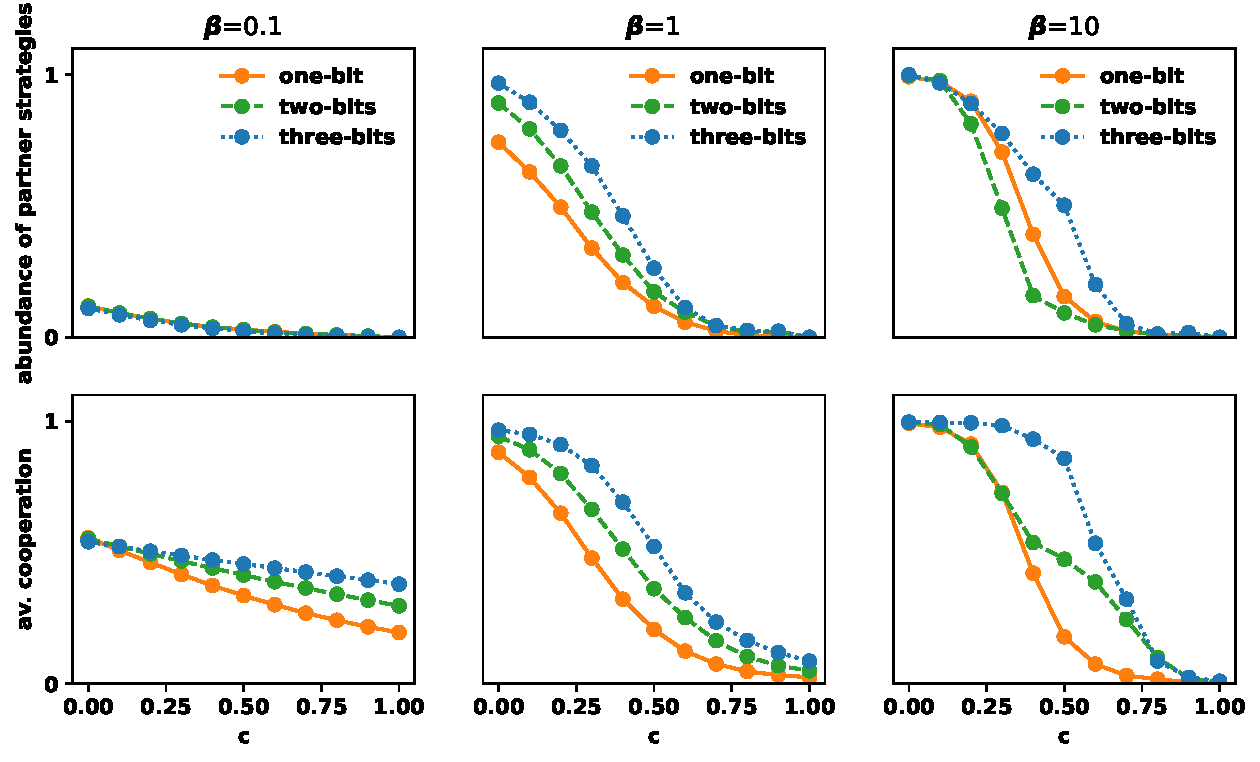
\includegraphics[width=\textwidth]{figures/abundance_of_partner_strategies.pdf}
%   \caption{The abundance of partner strategies for $n=1,2,3$ and $b=1, c=0.5$.}
% \end{figure}

% \begin{figure}[!htbp]
%   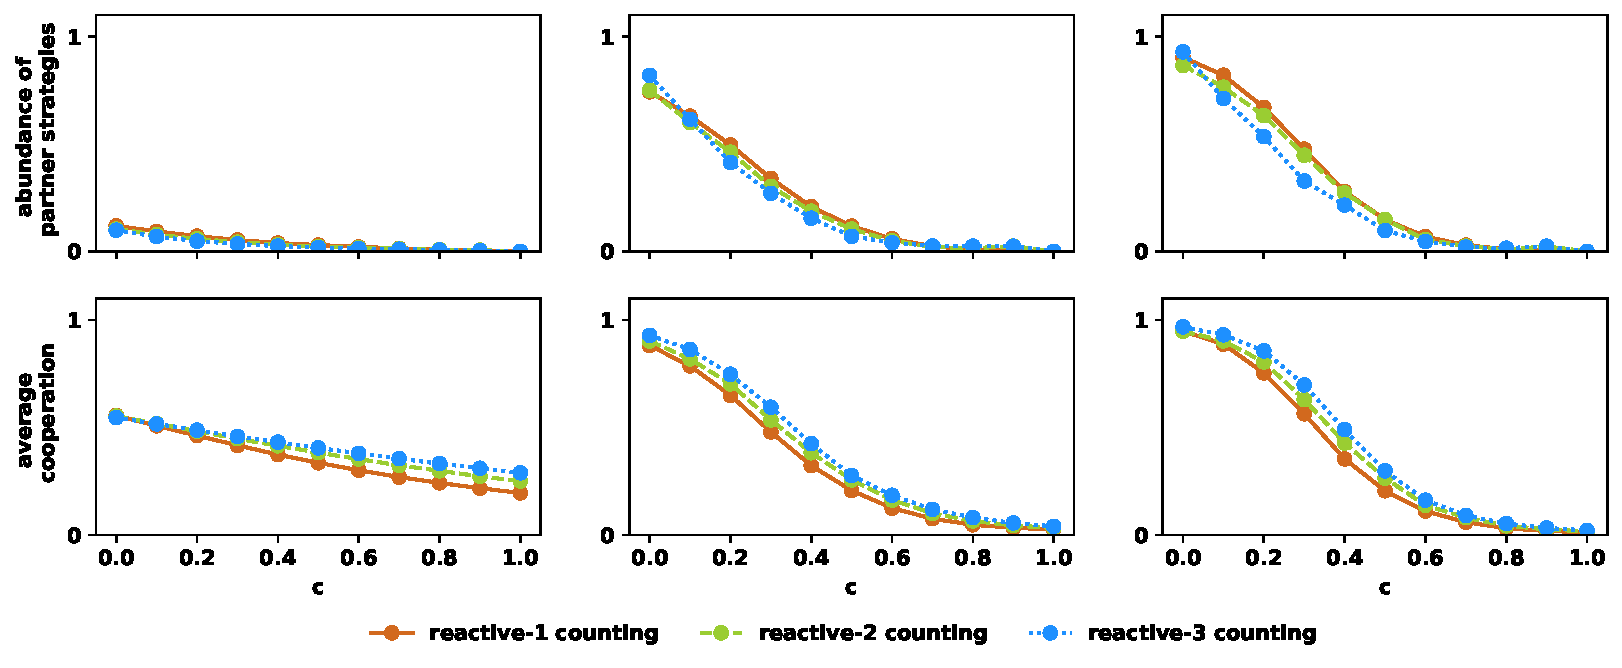
\includegraphics[width=\textwidth]{figures/abundance_of_partner_counting_strategies.pdf}
%   \caption{The abundance of partner counting strategies for $n=1,2,3$ and $b=1, c=0.5$.}
% \end{figure}

% \begin{figure}[!htbp]
%   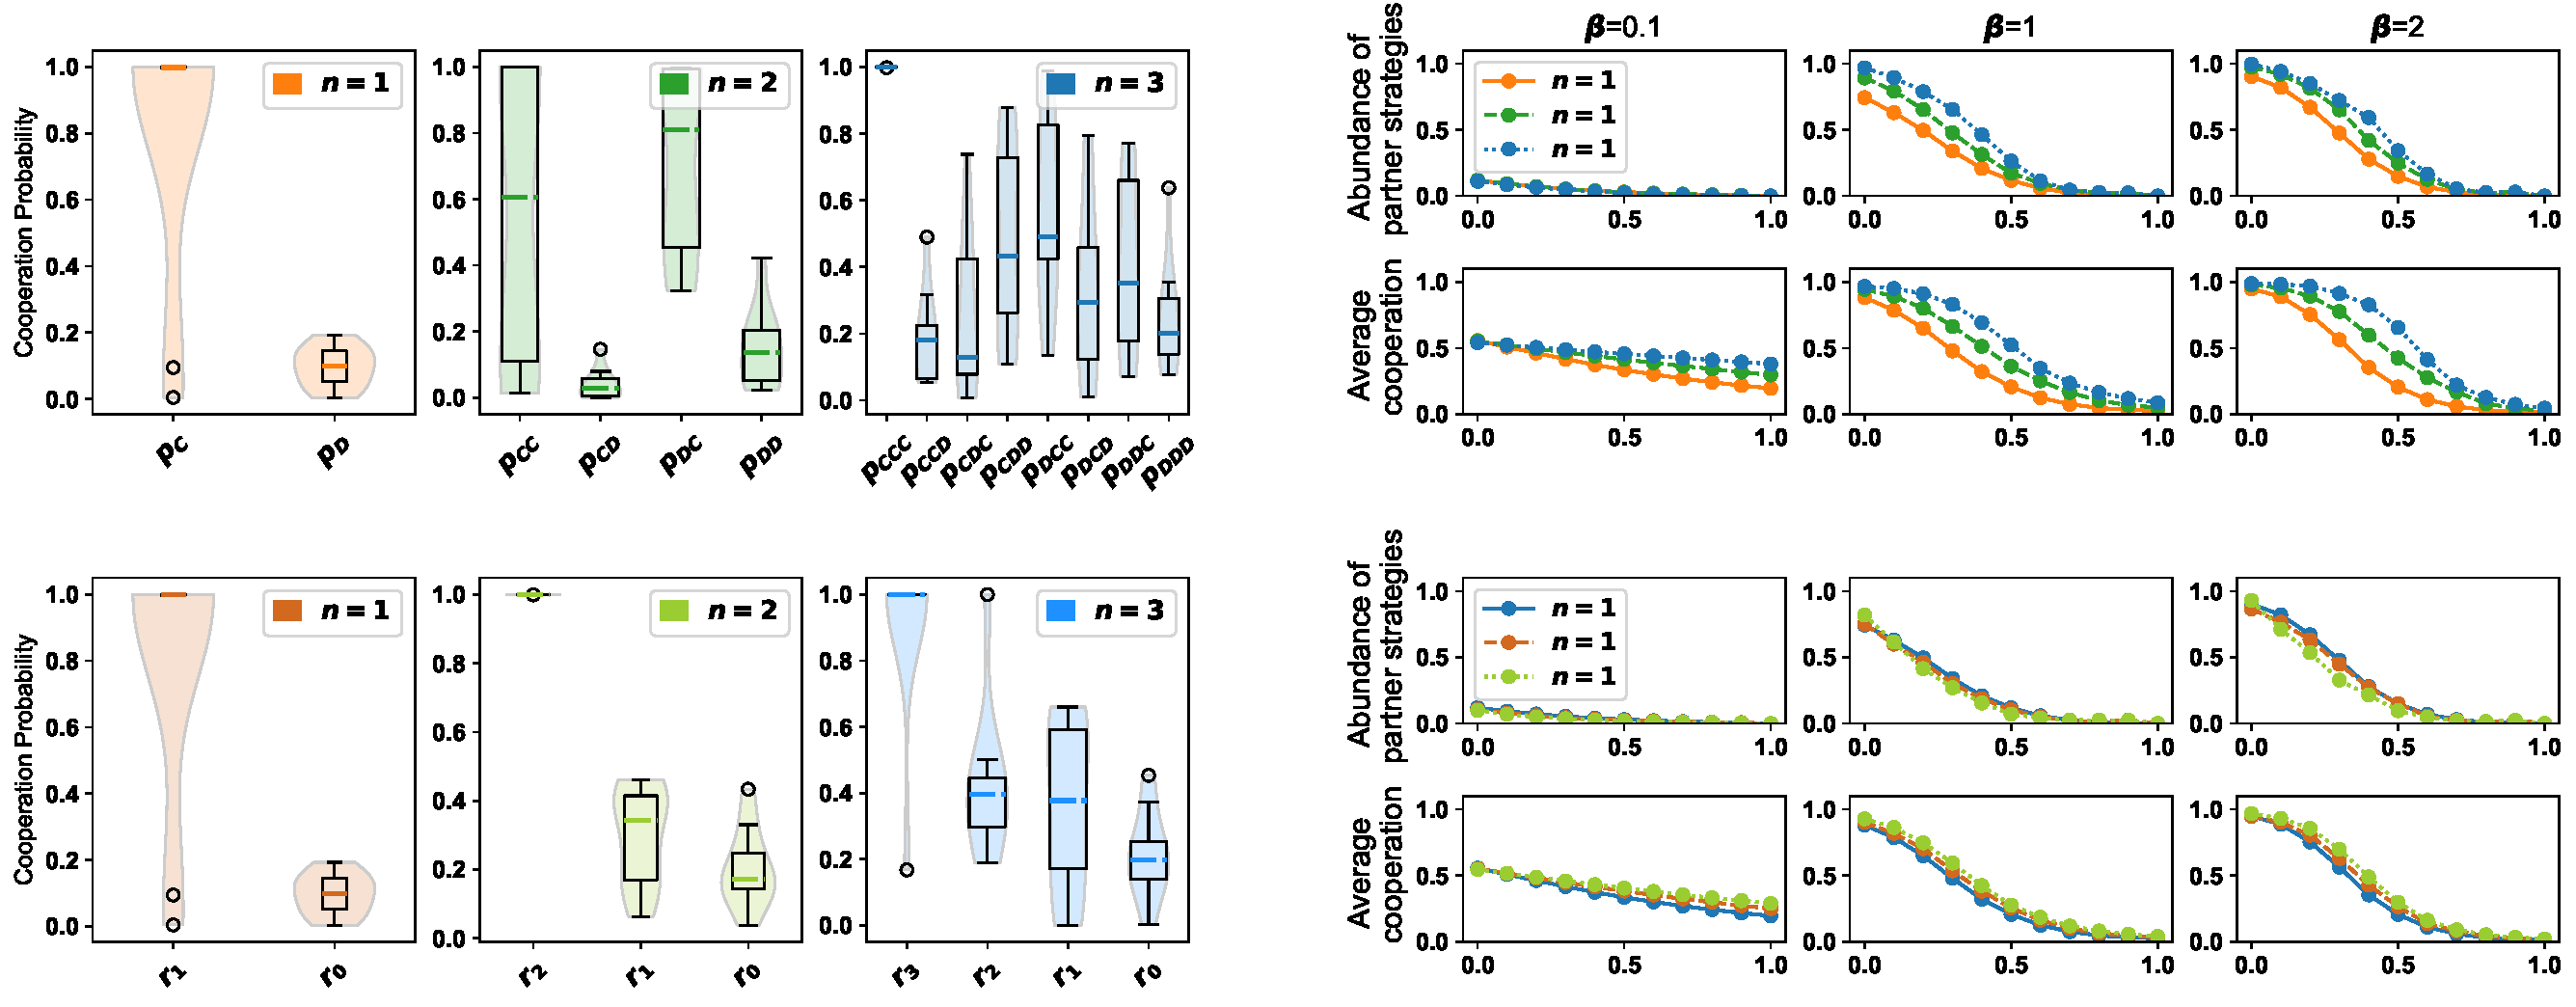
\includegraphics[width=\textwidth]{figures/abundant_strategies.pdf}
%   \caption{The most abundant reactive-$n$ strategies for $n=1,2,3$ and $b=1, c=0.5, \beta=1$.}
% \end{figure}

% \begin{figure}[!htbp]
%   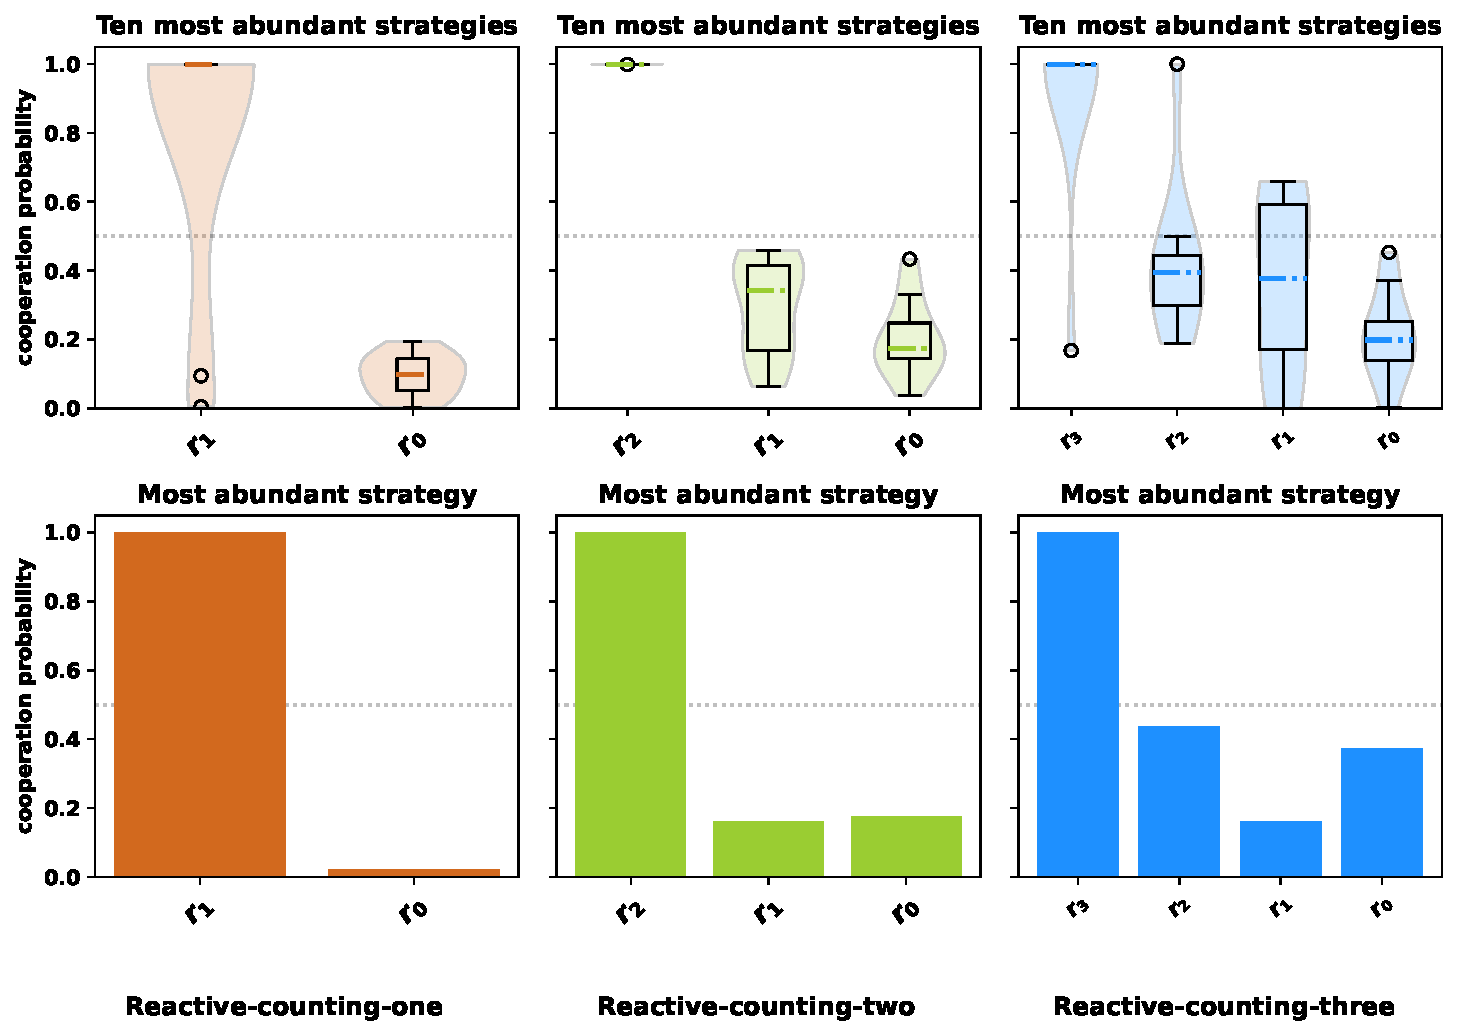
\includegraphics[width=\textwidth]{figures/abundant_strategies_counting.pdf}
%   \caption{The most abundant reactive-counting-$n$ strategies for $n=1,2,3$ and $b=1, c=0.5, \beta=1$.}
% \end{figure}

% % \begin{figure}
% %   \includegraphics[options]{fig}
% % \end{figure}

\section{Pure Self-Reactive-Three Strategies}\label{section:pure_self_reactive_n3}

The 256 pure self-reactive-three strategies and their vectors are as follows,

\begin{multicols}{3}
\input{figures/static/pure_self_reactive_n_3.txt}
\end{multicols}

~\\
\bibliography{bibliography.bib}

\end{document}